% !TEX root = main.tex

\section{Experimental Evaluation}\label{sec:experiments}


\begin{table*}[t]
	\large
	\centering
	\caption{Runtimes for four case studies.
		\textmd{Run times (in seconds) for computing open-loop controllers over the corresponding product spaces using ALTRO ($T_{g}^{\mathit{plan}}$), 
	number of state-input pairs of the finite abstraction for the largest ABCD task ($N_l$), 
	abstraction and synthesis times in SCOTS for that task (respectively $T_{l}^{\mathit{abs}}$ and $T_{l}^{\mathit{syn}}$), 
	number of state-input pairs of the finite state abstraction for global ABCD ($N_g$), 
	abstraction and synthesis times for computing a global controller for the product system using SCOTS 
	(respectively $T_{g}^{\mathit{abs}}$ and $T_{g}^{\mathit{syn}}$). ``OOM'' denotes ``out of memory'' on a 1.5TB RAM machine.
	}
		\label{tab:runtimes}
	}

	\renewcommand{\arraystretch}{1.1}
	%\setlength{\tabcolsep}{0.7em} % for the horizontal padding
	%\resizebox{1\columnwidth}{!}{
		\begin{tabular}{| l | S |S[table-format=+1.2e+1] S S|S[table-format=+1.2e+3] c c|}
			\hline
			Case-study	&	{Global planning}	&
			\multicolumn{3}{c|}{Local ABCD}	&	\multicolumn{3}{c|}{Global ABCD}\\
			
			&$T_{g}^{\mathit{plan}}$	&	$N_l$	&	$T_{l}^{\mathit{abs}}$	&	$T_{l}^{\mathit{syn}}$	&	$N_g$	&	$T_g^{\mathit{abs}}$	&	$T_g^{\mathit{syn}}$\\
			\hline
			
			Multi-drone path planning & 77.85 & 1.13e8 & 30.75  & 6.66	& 2.70e110	&	OOM	&	OOM \\
			
			\hline
			
			Crane and vehicle & 	0.65 & 8.56e8	&	511.24  & 91.43	&	2.16e18	&	OOM	&	OOM\\
			
			\hline
			
			Lane merging & 89.02 & 1.07e8	&	22.79  & 5.29	&	1.69e59	&	OOM	&	OOM\\
			\hline
			Multi-drone formation control & 114.34 & 1.55e8	&	39.46  & 7.83	&	3.65e50	&	OOM	&	OOM\\
			\hline
	\end{tabular}%}
\end{table*}

We have implemented our approach (as presented in Sec.~\ref{sec:problem}) in the open source tool \tool.\footnote{
	\tool is available online: https://github.com/MehrdadZareian/GAMARA.
}
We evaluate the effectiveness of \tool on two distinct categories of problems: 
local reach-avoid problems with collision avoidance and global formation control problems. 
We consider four case studies: multi-drone path planning, crane and vehicle, lane merging, and multi-drone formation control. 
The design of nominal controller using ALTRO for all experiments was performed on a machine with core i5-4590 CPU at 3.30GHz, with 16GB of RAM.
The formal controller synthesis using SCOTS for all systems except crane system was performed on the same machine. Controller synthesis for crane system is done on a cluster with 4 Intel Xeon E7-8857 v2 CPUs (48 cores in total) at 3GHz, with 1.5TB of RAM. 

%In all of our case studies, robots are moving in a two-dimensional space that has obstacles. 
%\KM{@Mehrdad: this sentence is not true for the crane.}
In all of our case studies, the robots are moving in a two-dimensional shared workspace (related but not exactly the same as the robots' state spaces) that possibly has obstacles. 
Table~\ref{tab:runtimes} shows run times for different stages of each experiment. 
For local ABCD, the reported numbers correspond to the maximum value among all of the agents. 
This choice is due to the fact that feedback controllers for different agents can be computed independently 
in parallel over different machines. 
To provide a more fine-grained comparison,
Fig.~\ref{fig:box_plot} shows the variations of run times of the different local ABCD tasks for every experiment. 
We have excluded the crane and vehicle case study in the figure due to an expected large variance originating from different dynamics. 
Notice that a higher number of state-input pairs does not necessarily result in a higher run time for local ABCD as the 
number of transitions and features of the parallel implementation can play a role. 
%
We compare \tool with ABCD applied to the product system to satisfy the global specification. 
As reflected in Table~\ref{tab:runtimes}, memory requirement for global ABCD exceeds both system's 
(laptop and cluster) limit (1.5TB of RAM) in all of the experiments.
%
%\begin{huge}
%
\begin{figure}[t]
	\centering
	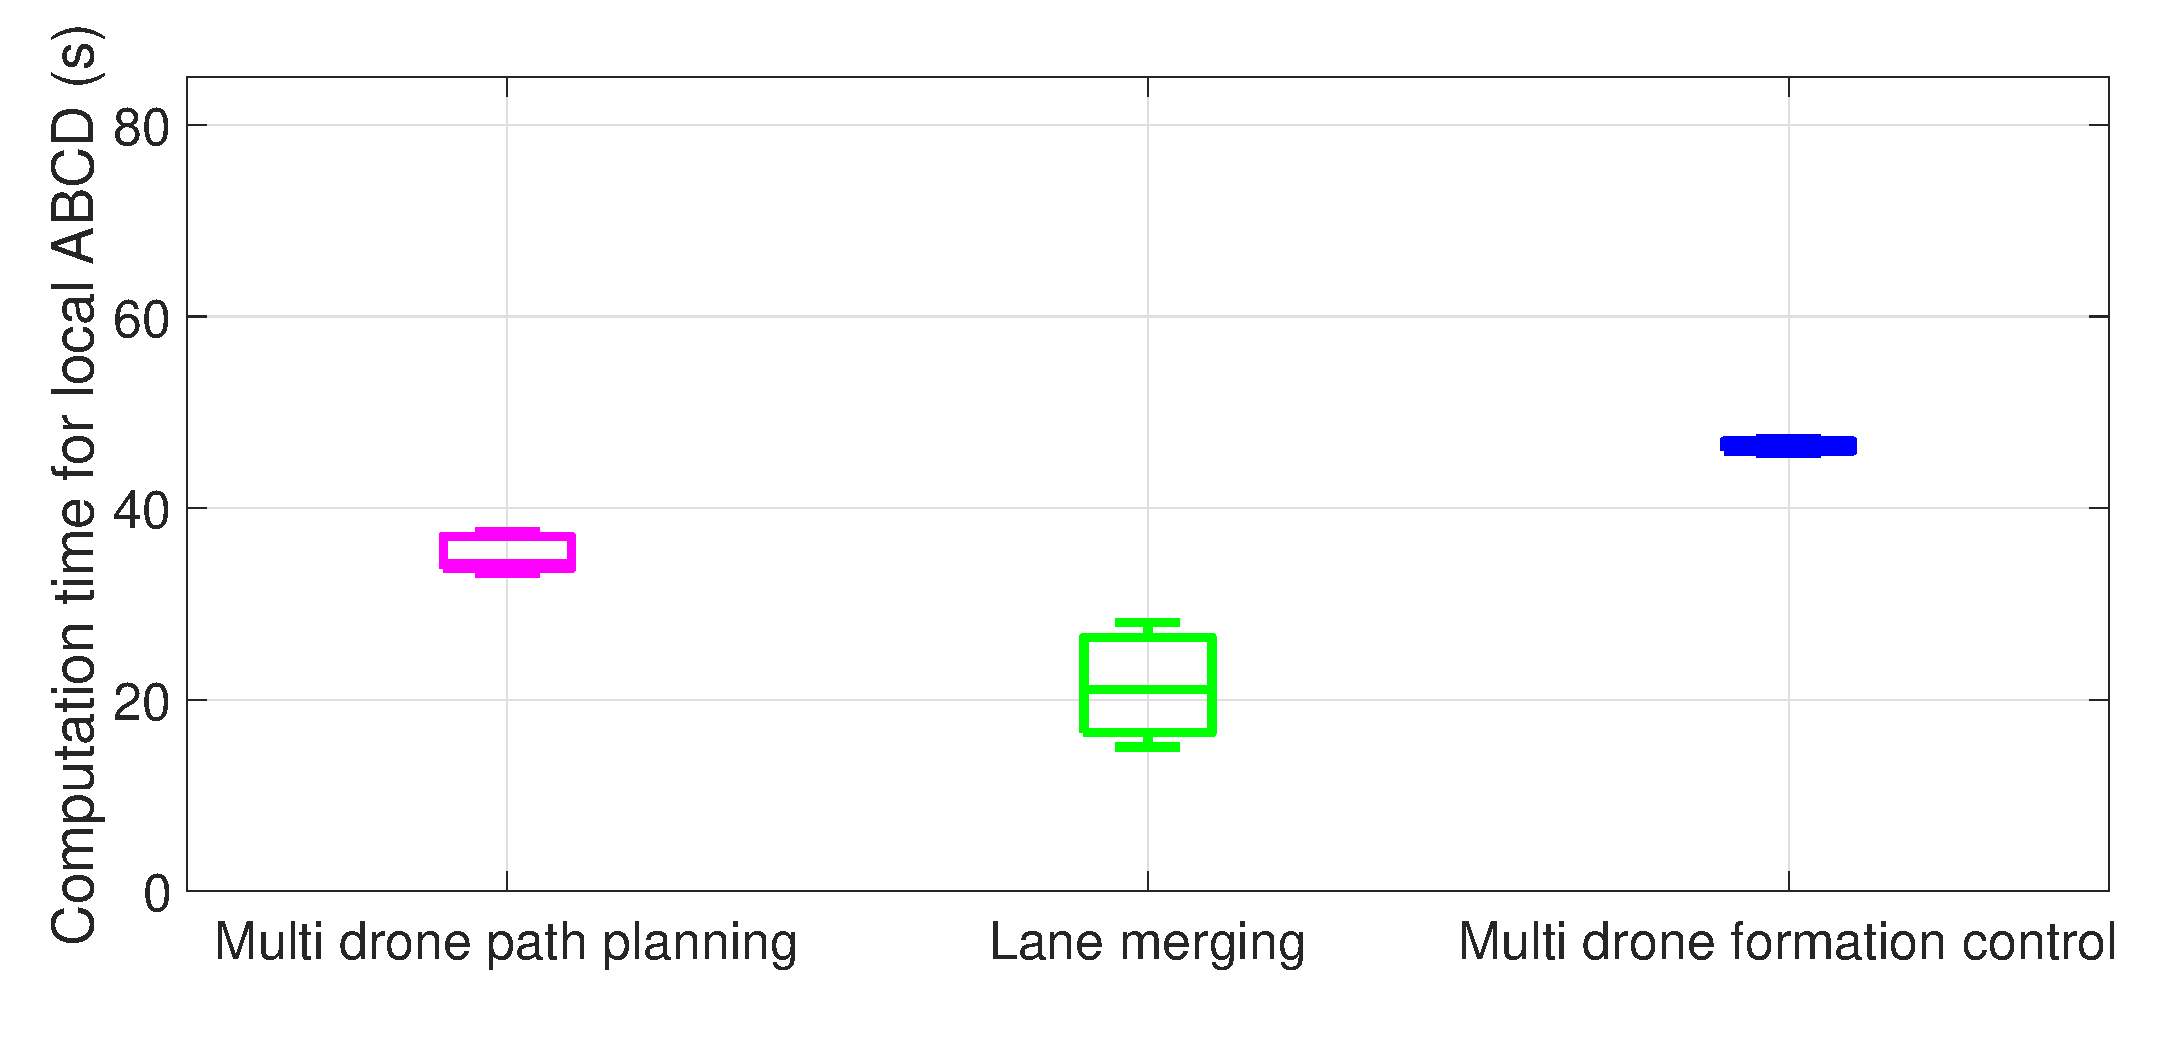
\includegraphics[width=\columnwidth]{figures/final_box_plot.eps}
	\caption{Variations of run times of local ABCD among different agents for three case studies.}
	\label{fig:box_plot}
	\vspace{-.3cm}
\end{figure}
%
\begin{figure}[t]
    \large
     \centering
         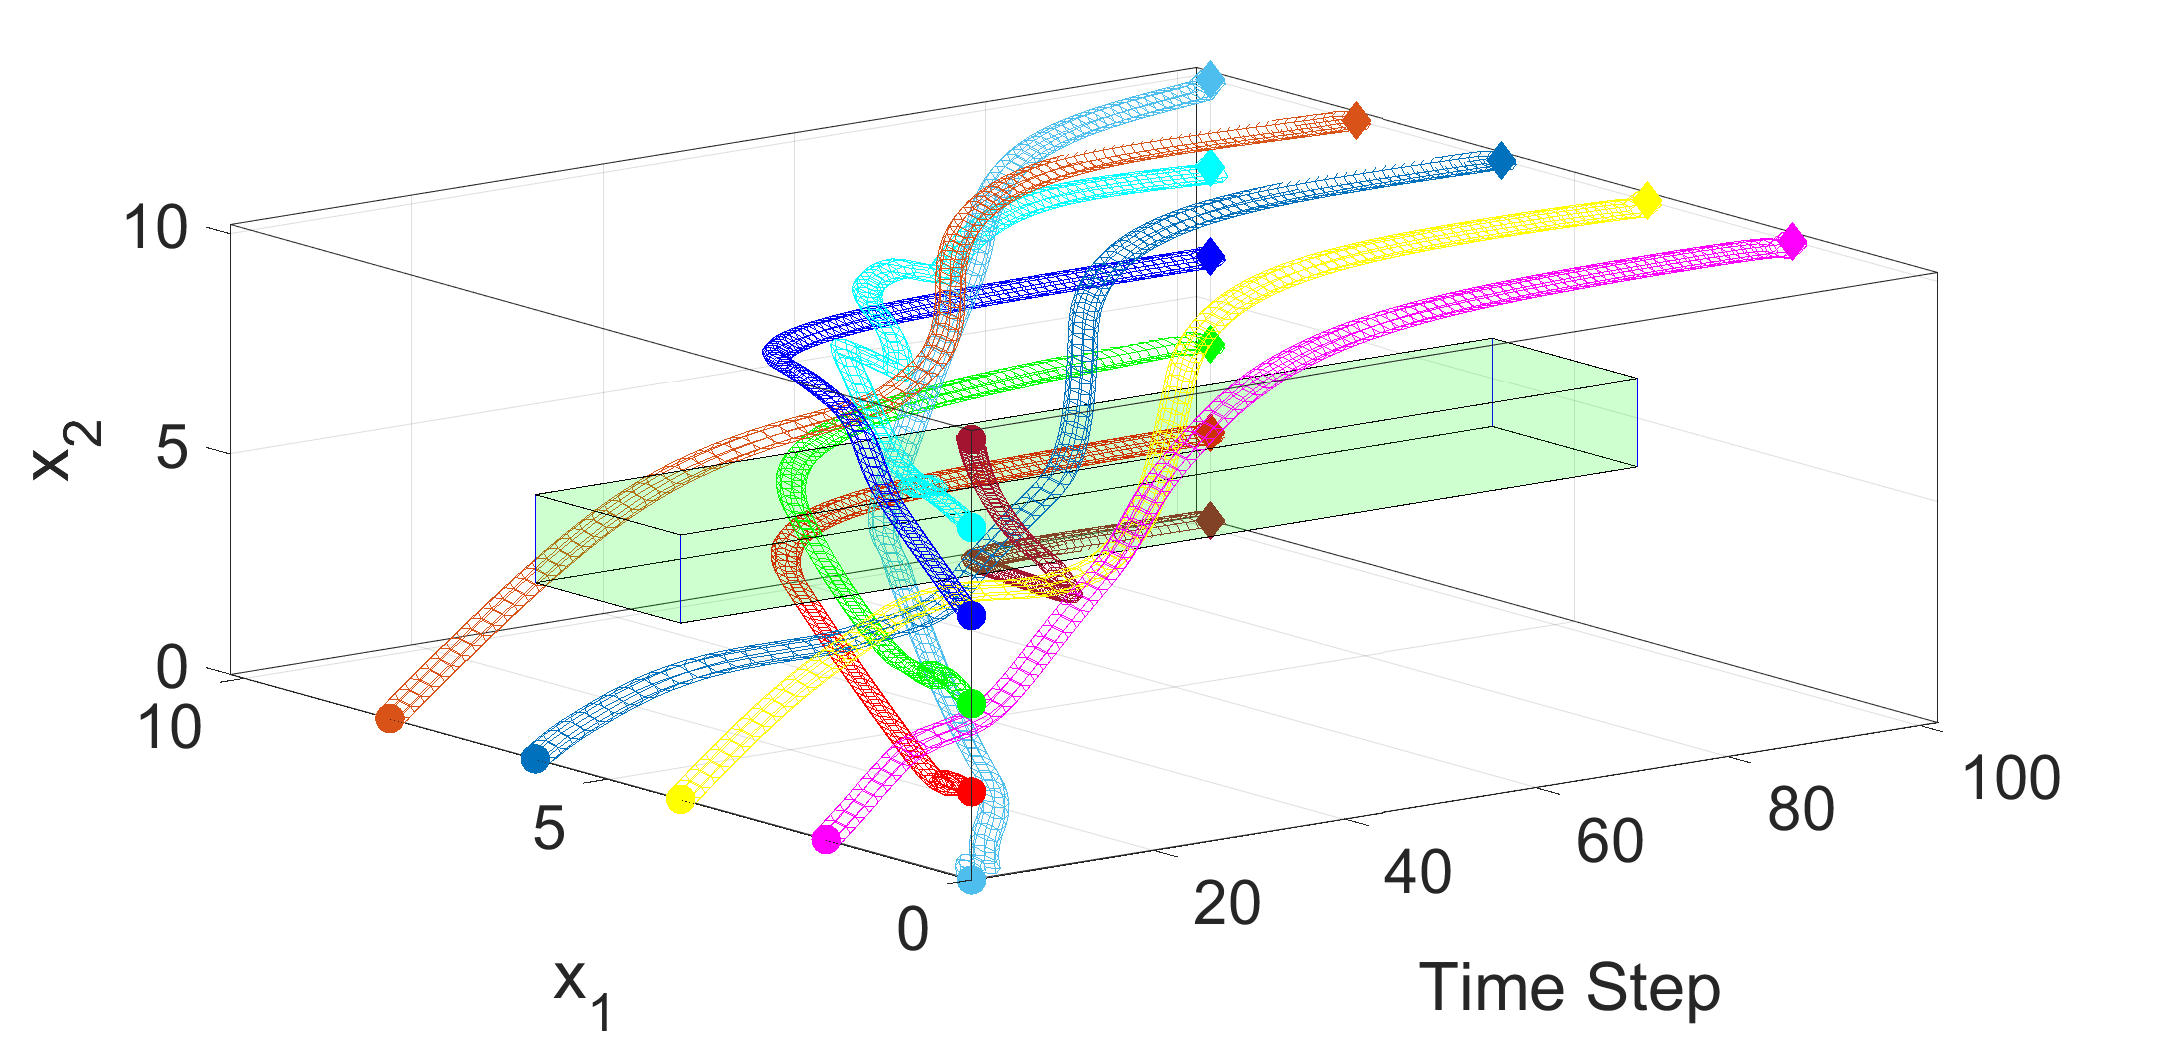
\includegraphics[width=\columnwidth]{figures/10t_final.eps}
        \caption{Time-state space illustration of tubes enclosing nominal trajectories for the multi-drone path planning}
        \label{fig:3dtubes}
        \vspace{-.3cm}
\end{figure}

%\end{huge}
\subsection{Local reach-avoid with collision avoidance}
\label{sec:local reach-avoid}
%
We first consider situations when each robot has an individual reachability specification, 
and they need to ensure a minimum safe distance from each other and the obstacles.
% We show how this case can be captured using the problem description outlined in Sec.~\ref{sec:problem}.

Suppose $\set{\Sigma^i}$ 
% with $\Sigma^i=(X^i,x_\init^i,U^i,W^i,f^i)$ 
models a set of robots, 
$\goal^i\subseteq X^i$ are the individual goal sets, and $\delta \in \mathbb{R}_{>0}$ is a safety margin for collisions. 
We consider each robot as a point object with a bounding box for its physical dimensions. 
The parameter $\delta$ is chosen to be a constant greater than \new{twice} the radius of the bounding box around each robot. 
By keeping a distance at least $\delta$ from the other robots and the obstacles, the robots can avoid collision in their physical domain.
The parameter $\delta$ can additionally take into account statutory minimum safe distances among the robots, 
such as in autonomous driving-like scenarios.
The choice of $\delta$ is completely independent of the choice of $\varepsilon$. 
The latter is a robustness margin introduced to take into account the deviation of the system trajectories under external disturbances.
Suppose the specification requires that each robot $\Sigma^i$ eventually reaches $\goal^i$ 
while avoiding the obstacle $\obs\subseteq \reals^2$ and collision with robots by the margin $\delta$.
The global specification on the product system $\Sigma^\times$ 
is as follows:
\begin{itemize}
	\item The goal set $\goal\subseteq X^\times$ is defined as $\goal \coloneqq \goal^1\times \ldots \times \goal^N \subseteq X^\times$, and
	\item The avoid set $\avoid\subseteq X^\times$ is defined as 
		\begin{align}
% 			&\avoid \coloneqq\nonumber\\ 
				&\Set{ x^\times\in X^\times | 
					\begin{array}{c}
						\exists i\in [1;N]\;.\; d_\obs(x^i,\obs) \leq \delta\\
						\vee\\
						 \exists i,j\in [1;N]\;.\;i\neq j\;.\;d_\col\left(x^i,x^j\right)\leq\delta
					\end{array}},
		\end{align}
	where $x^i$ denotes the component of $x^\times$ corresponding to $\Sigma^i$, $d_\col(\cdot,\cdot)$ denotes a 
distance metric for measuring the geometric distance between positions of two systems located in two-dimensional space, 
and $d_\obs(\cdot,\cdot)$ denotes a distance metric for measuring the geometric distance between the 
position of one system and the obstacle $\obs\subseteq \reals^2$.
\end{itemize}
%

In this category of problems, we apply our approach to three case studies as briefly discussed next. 
The detailed models for the systems and their different parameters have been presented in Sec.~\ref{sec:Multirobot}-\ref{sec:lane merging} in the appendix, and the performance of \tool for these experiments have been summarized in the first three rows on Table~\ref{tab:runtimes}.

\subsubsection{Multi-drone path planning}\label{subsec:Multirobot}
We consider a planning scenario for ten identical drones ($N=10$). 
The control objective is to synthesize a feedback controller for each drone so that in the presence of (bounded) disturbance, beginning from the specified initial state, the corresponding target state is reached within a finite horizon, 
while avoiding collision with other drones and the physical obstacle at every time point. 
Fig.~\ref{fig:3dtubes} gives a time-space illustration for the safe tubes around the nominal trajectories. 
The tracking feedback controllers are synthesized such that every drone remains within its safe tube until reaching its destination, 
even with worst-case disturbance.  
Additional analysis and detailed models for the systems and their different parameters are presented in Sec.~\ref{sec:Multirobot} in the appendix.

\subsubsection{Crane and Vehicle}
The goal of this example is to study the performance of our method for 
controlling a number of robots with different dynamics. 
As described in Sec.~\ref{sec:intro}, the goal is to move the overhead crane
and the vehicle such that they do not collide.
Formally guaranteed controllers are computed such that the generated open loop trajectory 
(see Fig.~\ref{fig:cr_and_lft} (\textbf{left})) is tracked even under disturbance. 
More detailed discussion on dynamics of systems and further analysis are presented in Sec.~\ref{subsec:crane_vehicle} in the appendix.

\subsubsection{Lane Merging}
\label{subsec:lane merging}
We study a lane merging problem wherein multiple \RM{What is $N$?}
controlled vehicles are driving over two merging lanes (Fig.~\ref{fig:merge}, \textbf{top} frame). 
A dangerous situation may occur at the merging point of the two lanes if vehicles are not controlled properly. 
Different variants of this problem have been studied in the literature (see, e.g., \cite{xiao2019merging,xiao2020merging}). Without seeking to optimize fuel consumption or travel time, we set the goal to control the vehicles to pass the merging zone safely. In particular, consider a situation where initially three cars are driving on each of the two lanes (Fig.~\ref{fig:merge}, (\textbf{top})). The control objective for each vehicle is to pass the red dashed line within a finite horizon without hitting the road's sides or colliding with other vehicles. Fig.~\ref{fig:merge} demonstrates snapshots of one sample trajectory when feedback controllers are employed under the presence of bounded disturbance. Additional analysis, systems' dynamics and parameters are reported in Sec.~\ref{sec:lane merging} in the appendix.
\begin{figure}
	\centering
	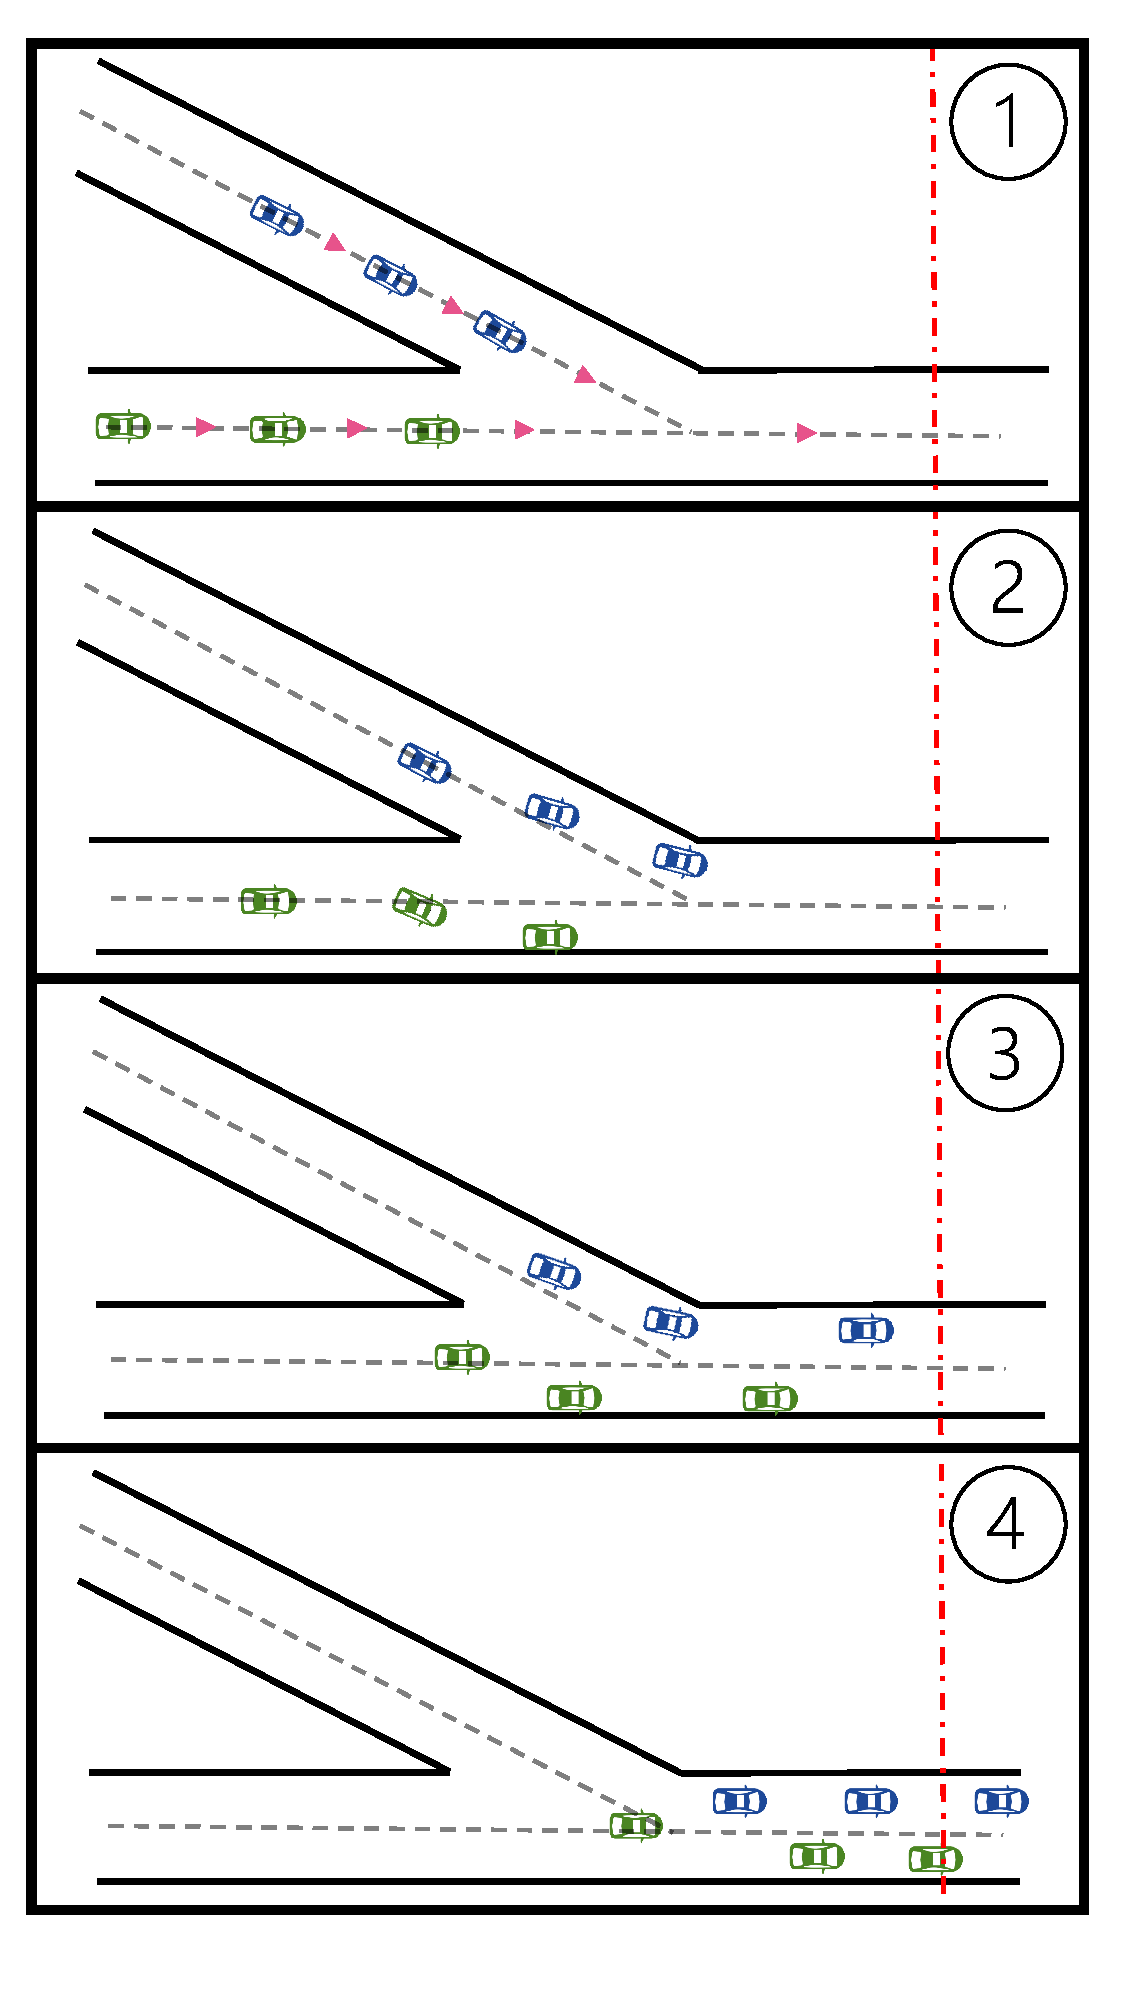
\includegraphics[scale=.21]{figures/merge_updated.pdf}
	\caption{Illustration of a sample trajectory generated by formally guaranteed controllers for the lane merging example}
	\label{fig:merge}
\vspace{-0.4cm}
\end{figure}


\subsection{Global formation control problem}\label{sec:global formation control}

The second category of examples are about maintaining a global formation while satisfying a set of reach-avoid specifications.
We show how the formation control problem can be expressed using a static obstacle $\avoid$ on the product state space $X^\times$.

Let us first formalize the notion of \emph{formation}.
Let $\Set{\Sigma^i=(X^i,x_\init^i,U^i,W^i,f^i)}$ be a set of robots.
A \emph{formation constraint} is a set $\Set{\lambda^{i,j}\in \mathbb{R}}_{i,j\in [1;N]}$ where every $\lambda^{i,j}$ specifies the relative \emph{Euclidean} 
distance between the projections of state of robot $\Sigma^i$ and robot $\Sigma^j$.%\RM{undef:} over the shared output space $Y$.
%(We use euclidean distance to define formation, as opposed to the distance $D$ used in the rest of the paper, to allow rotation of the formation while moving.)

Now suppose $\goal^i\subseteq X^i$ are the individual goal states, $\obs\subset \reals^2$ is a common obstacle % in the \RM{undef:} output space, 
$\delta \in \mathbb{R}_{>0}$ is a safety margin, and $\mu\in \mathbb{R}_{>0}$ is a tolerance margin for the formation constraint.
The formation control problem then asks to generate controllers $\set{C_i}$ such that every robot $\Sigma^i$ eventually reaches $\goal^i$ while avoiding $\obs$ 
by the margin $\delta$, as well as while making sure that the \emph{Euclidean} distance between robots $\Sigma^i$ and $\Sigma^j$ is in the range $\lambda^{i,j} \pm \mu$.
Essentially the tolerance margin $\mu$ is to account for the possible slight deviations due to disturbances experienced by the robots. 
Notice that since the robots have their own goals but at the same time they need to ``stay close'' to their neighboring robots in the formation for the entire period, 
they might first need to accompany the other robots to their goals, before being accompanied by them to reach their own goal.
%
We can express the formation control problem in the product state space as follows:
\begin{itemize}
	\item The goal set $\goal\!\subseteq\! X^\times$ is defined as $\goal\!\coloneqq\! \goal^1\!\times \ldots \times\! \goal^N$, and
	\item The avoid set $\avoid\subseteq X^\times$ is 
		\begin{align}
%			&\avoid \coloneqq\nonumber\\ 
			&\Set{ x^\times\in X^\times | 
				\begin{array}{c}
					\exists i\in [1;N]\;.\; D(x^i,\obs) \leq \delta\\
					\vee\\
					\exists i,j\in [1;N]\;.\; i\neq j\;.\; d\left(x^i,x^j\right)\notin\lambda^{i,j}\pm \mu
			\end{array}},					
		\end{align}
\end{itemize}
where the last disjunction in the definition of $\avoid$ is the restriction required for maintaining the formation, and the rest are 
same as in Sec.~\ref{sec:local reach-avoid}.

\subsubsection{Multi-drone formation control}
\label{subsec:formation_control}
Consider a formation control scenario where a set of five drones (identically modeled) need to go from a specified start point to a certain destination (both defined over the corresponding state spaces) within a finite horizon, while four of them forming a diamond around a fifth drone (positioned at the diamond's center) at every time point. There are two square obstacles from which the group needs to keep a certain minimum distance at all of the time points. Fig.~\ref{fig:formation_ex} illustrates four sequential frames of a sample perturbed trajectory generated by employing formally guaranteed feedback controllers. Notice that both 
relative position and orientation between drones are kept (almost) constant 
throughout the journey. 
Further analysis can be found in Sec.~\ref{sec:formation_control} in the appendix.
%
 \begin{figure}[t]
	\centering
	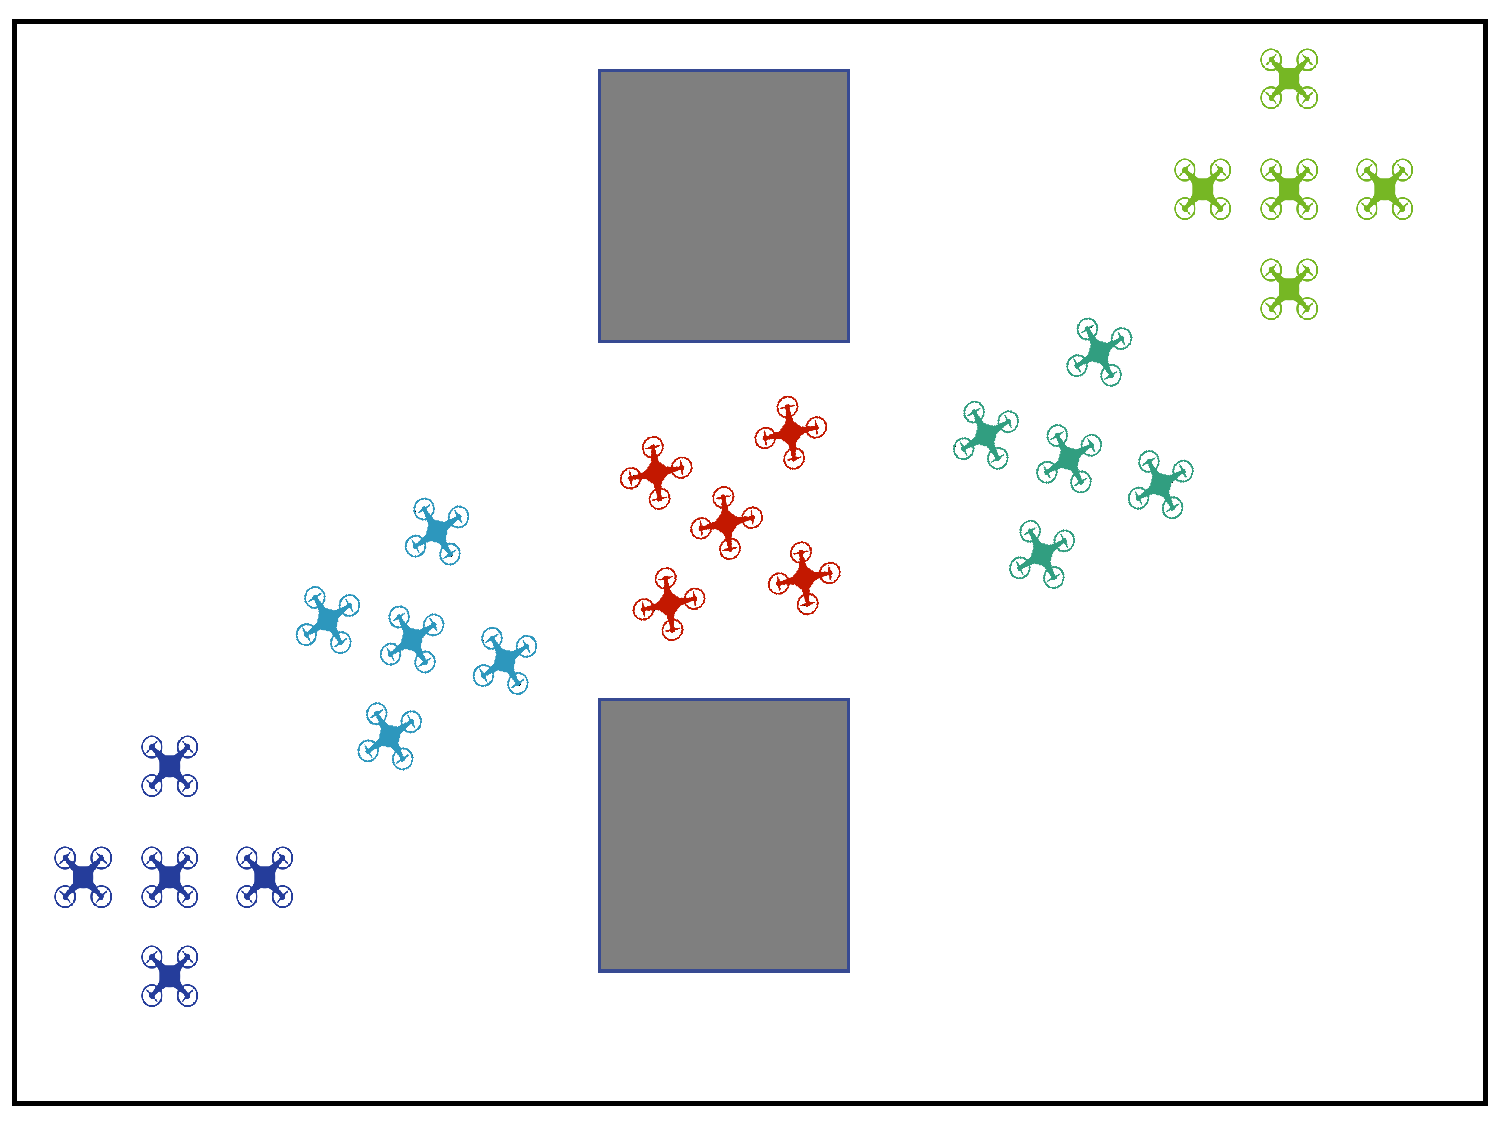
\includegraphics[scale=0.22]{figures/formation.pdf}
	\caption{Illustration of a sample trajectory generated by the feedback controllers for the formation control example}
	\label{fig:formation_ex}
	\vspace{-.4cm}
\end{figure} 

%Note that $\delta_{col} > \varepsilon$.
%We use SCOTS in order to synthesize (local) feedback controllers that guarantee reachability, formation control and obstacle/collision avoidance in the presence of bounded disturbance such that $|W|\leq \begin{bmatrix}??&??&??\end{bmatrix}^T$. 
%We consider state and input spaces to be $X=[??:??]^2\times[??,??]$ and
%$U=[??,??]^2$, respectively. Choosing state and input partition sizes $\eta_{X}=[??,??,??]^T$ and
%$\eta_{U}=[??,??]^T$ results in $\hat X$ and $\hat U$ with $??\times ??$ and $??$ points. As we explained in Sec.~\ref{sec:tracking}, we compute the transition system over inter-tube space which has $|\hat P|=??\times ??$ points in this example.%The bound over additive disturbance is set to be $\begin{bmatrix}0.03&0.03&0.03&0\end{bmatrix}^T$. 
%Given the above settings, SCOTS computes abstraction in $??$ minutes for all the drones and synthesizes controllers in about $??$ minutes (in average, abstraction takes $??$ seconds and synthesis takes $??$ seconds). 
%\section{Present Challenges}
%
%\begin{enumerate}
%	\item In some examples, it was necessary to consider a larger control input space for the SCOTS part, than what was used in the ALTRO part.
%	Otherwise, the SCOTS would not be able to track the nominal trajectory within the given precision using any level of discretization. 
%	\item For the ship example, applying the largest disturbance with which SCOTS is able to compute a controller, the trajectory resulted from using the open loop controller does not leave  $\varepsilon-$tube around it; in general magnitude of disturbance for which SCOTS can find a controller is relatively small for most of examples that we have tried.
%\end{enumerate}









